% =============================================================================
% Supplementary Materials for BIB submission
% Paired prediction of GPCR-G protein coupling specificity
% =============================================================================

\documentclass[11pt,a4paper]{article}
\usepackage[margin=2.5cm]{geometry}
\usepackage{times}
\usepackage{natbib}
\usepackage{graphicx}
\usepackage{amsmath,amssymb}
\usepackage{booktabs}
\usepackage{caption}
\usepackage{hyperref}
\usepackage{float}
\usepackage[font=small,labelfont=bf]{caption}
\usepackage{multirow}

\hypersetup{colorlinks=true, citecolor=blue, linkcolor=black, urlcolor=blue}

\makeatletter
\renewcommand{\@maketitle}{%
  \newpage\null\vspace{-2em}%
  {\LARGE\bfseries Supplementary Materials\par}%
  \vskip 0.5em%
  {\Large\bfseries Paired prediction of GPCR--G protein coupling specificity\par}%
  \vskip 1.5em%
  {\large
   \begin{center}%
     Guohao Lv\textsuperscript{1},\ \ Yingchun Xia\textsuperscript{1},\ \ Huichao Liu\textsuperscript{1},\ \ Xiaolei Zhu\textsuperscript{1,2},\\[0.1em]
     Shuai Yang\textsuperscript{1,2},\ \ Qingyong Wang\textsuperscript{1,2,*},\ \ Lichuan Gu\textsuperscript{1,2,*}
   \end{center}%
  \par}%
  \vskip 1em%
}
\makeatother
\title{}
\author{}
\date{}

\begin{document}
\maketitle

% =============================================================================
\section{Supplementary Tables}

\begin{table}[h!]
\centering
\caption{Complete AlphaFold structural descriptors (38 features). All features are derived from predicted \textbf{monomer} GPCR structures (AlphaFold2). G$\alpha$-contact residues are mapped from known GPCR--G protein complex templates (rhodopsin--G$\alpha$t, $\beta_2$AR--G$\alpha$s) and should be interpreted as \textbf{intracellular-interface proxy features}, not complex-derived descriptors.}
\label{tab:alphafold_features}
\begin{tabular}{lll}
\toprule
Category & Descriptor & Dimension \\
\midrule
\multirow{2}{*}{TM distances} & TM5--TM6 cytoplasmic C$\alpha$ distance & 1 \\
                              & TM3--TM6 cytoplasmic C$\alpha$ distance & 1 \\
\midrule
\multirow{2}{*}{ICL geometry} & ICL2 end-to-end C$\alpha$ distance & 1 \\
                              & ICL3 end-to-end C$\alpha$ distance & 1 \\
\midrule
\multirow{4}{*}{Dihedral angles} & Mean $\phi$ (ICL2) & 1 \\
                                 & Mean $\psi$ (ICL2) & 1 \\
                                 & Mean $\phi$ (ICL3) & 1 \\
                                 & Mean $\psi$ (ICL3) & 1 \\
\midrule
\multirow{6}{*}{Intracellular-interface SASA (proxy)} & Total intracellular SASA & 1 \\
                                & ICL2 SASA & 1 \\
                                & ICL3 SASA & 1 \\
                                & TM5 cytoplasmic-tip SASA & 1 \\
                                & TM6 cytoplasmic-tip SASA & 1 \\
                                & Template-mapped G$\alpha$-contact SASA\textsuperscript{*} & 1 \\
\midrule
\multirow{6}{*}{DSSP ratios} & Helix ratio (ICL2) & 1 \\
                             & Strand ratio (ICL2) & 1 \\
                             & Coil ratio (ICL2) & 1 \\
                             & Helix ratio (ICL3) & 1 \\
                             & Strand ratio (ICL3) & 1 \\
                             & Coil ratio (ICL3) & 1 \\
\midrule
\multirow{8}{*}{PAE features (monomer)} & Mean PAE (TM5--TM6) & 1 \\
                              & Max PAE (TM5--TM6) & 1 \\
                              & Mean PAE (ICL2--TM5/TM6 intracellular) & 1 \\
                              & Max PAE (ICL2--TM5/TM6 intracellular) & 1 \\
                              & Mean PAE (ICL3--TM5/TM6 intracellular) & 1 \\
                              & Max PAE (ICL3--TM5/TM6 intracellular) & 1 \\
                              & Mean PAE (TM5--template G$\alpha$-contact residues)\textsuperscript{*} & 1 \\
                              & Mean PAE (TM6--template G$\alpha$-contact residues)\textsuperscript{*} & 1 \\
\midrule
\multicolumn{2}{l}{\textbf{Total}} & \textbf{38} \\
\bottomrule
\multicolumn{3}{p{0.88\textwidth}}{\small \textsuperscript{*}These features use G$\alpha$-contact residue positions mapped from template GPCR--G protein complexes. They describe the intracellular cavity of the monomer structure, not a modeled complex interface.} \\
\end{tabular}
\end{table}

\begin{table}[h!]
\centering
\caption{Random 5-fold cross-validation AUC (no cluster constraint).}
\label{tab:random_cv}
\begin{tabular}{lcccc}
\toprule
Model & Embedding & Baseline & +ICL & +ICL+AF \\
\midrule
SVM (RBF)       & 8M   & 0.8860 $\pm$ 0.0048 & 0.9233 $\pm$ 0.0021 & 0.9216 $\pm$ 0.0026 \\
SVM (RBF)       & 650M & 0.9044 $\pm$ 0.0036 & 0.9260 $\pm$ 0.0025 & 0.9244 $\pm$ 0.0034 \\
Cross-Attention & 8M   & 0.9031 $\pm$ 0.0065 & 0.9154 $\pm$ 0.0058 & 0.9132 $\pm$ 0.0061 \\
Cross-Attention & 650M & 0.9423 $\pm$ 0.0071 & \textbf{0.9695 $\pm$ 0.0049} & 0.9671 $\pm$ 0.0040 \\
MLP             & 650M & 0.9386 $\pm$ 0.0082 & 0.9668 $\pm$ 0.0044 & 0.9642 $\pm$ 0.0051 \\
\bottomrule
\end{tabular}
\end{table}

\begin{table}[h!]
\centering
\caption{Leave-one-G-protein-family-out (LOGPSO) AUC, per-family and mean.}
\label{tab:logpso}
\begin{tabular}{lccccc}
\toprule
Model & Gq & Gi & Gs & G12/13 & Mean \\
\midrule
SVM (RBF, 8M baseline)  & 0.549 & 0.628 & 0.510 & 0.591 & 0.570 \\
SVM (RBF, 650M + ICL)   & 0.585 & 0.674 & 0.527 & 0.637 & 0.606 \\
Cross-Attention (650M + ICL) & 0.578 & 0.671 & 0.523 & 0.633 & $\sim$0.601 \\
Multi-Task CA (650M)     & 0.567 & 0.658 & 0.514 & 0.624 & 0.591 \\
\bottomrule
\end{tabular}
\end{table}

\begin{table}[h!]
\centering
\caption{Hyperparameter configurations for all models.}
\label{tab:hyperparams}
\begin{tabular}{ll}
\toprule
Model & Hyperparameters \\
\midrule
SVM (RBF) & $C=10.0$, $\gamma=\text{scale}$, class\_weight=balanced \\
MLP & Hidden: [256,128,1], GELU, BN, Dropout=0.3, LR=$10^{-4}$, WeightDecay=$10^{-4}$ \\
Cross-Attention & Hidden=256, Heads=4, Layers=3, GELU, LayerNorm, Dropout=0.3 \\
Random Forest & n\_estimators=100, max\_depth=10, class\_weight=balanced \\
XGBoost & n\_estimators=100, max\_depth=6, LR=0.1, scale\_pos\_weight=balanced \\
\midrule
\multicolumn{2}{l}{\small All deep models: AdamW optimizer, BCELoss, batch\_size=32, max\_epochs=200,}\\
\multicolumn{2}{l}{\small early\_stopping\_patience=20, gradient\_clipping=1.0.}\\
\multicolumn{2}{l}{\small SVM and tree models: nested 3-fold inner CV for hyperparameter selection.}\\
\end{tabular}
\end{table}

\begin{table}[h!]
\centering
\caption{Promiscuity-stratified Cluster-CV AUC (cross-attention 650M + ICL). Values are per-fold mean $\pm$ standard deviation across five cluster-aware CV folds. Positive ratio varies across strata due to the differing number of positive pairs per promiscuity level.}
\label{tab:promiscuity_cv}
\begin{tabular}{lrrrrr}
\toprule
GPCR Promiscuity & N pairs & Pos. ratio & CA AUC & SVM AUC & $\Delta$AUC \\
\midrule
Single-family   & 616 & 0.157 & 0.8808 & 0.8659 & +0.0149 \\
Dual-family     & 321 & 0.412 & 0.7672 & 0.7724 & $-$0.0053 \\
Triple-family   & 107 & 0.664 & 0.7443 & 0.7334 & +0.0108 \\
\midrule
Overall (all GPCRs) & 1,639 & 0.254 & 0.8466 & 0.8309 & +0.0157 \\
\bottomrule
\multicolumn{6}{l}{\small AUC values computed on concatenated held-out test predictions from 5-fold cluster-aware CV.} \\
\multicolumn{6}{l}{\small Promiscuity defined as number of experimentally annotated G protein families per GPCR.} \\
\multicolumn{6}{l}{\small GPCRs with zero annotated couplings (orphans) are excluded from this stratified analysis.} \\
\end{tabular}
\end{table}

\begin{table}[h!]
\centering
\caption{Confidence-stratified prediction performance (cross-attention 650M + ICL, cluster-aware 5-fold CV).}
\label{tab:confidence}
\begin{tabular}{lrrr}
\toprule
Confidence threshold & Coverage (\%) & Accuracy (\%) & N predictions \\
\midrule
$\ge$ 0.50 & 92.7 & 83.3 & 1,519 \\
$\ge$ 0.70 & 90.1 & 84.1 & 1,477 \\
$\ge$ 0.80 & 85.8 & 85.3 & 1,407 \\
$\ge$ 0.90 & 79.4 & 86.5 & 1,302 \\
$\ge$ 0.95 & 73.2 & 87.6 & 1,200 \\
$\ge$ 0.98 & 63.8 & 89.0 & 1,046 \\
\bottomrule
\multicolumn{4}{l}{\small Confidence $= 2 \times |P(\text{coupling}) - 0.5|$. Coverage = fraction of all predictions.} \\
\multicolumn{4}{l}{\small Predictions are held-out test set predictions from 5-fold cluster-aware CV.} \\
\end{tabular}
\end{table}

\begin{table}[h!]
\centering
\caption{Cluster-aware precision-recall AUC (PRAUC) for primary model configurations. Random baseline PRAUC equals the positive class ratio (0.256 for the full dataset). All reported PRAUC values substantially exceed this baseline.}
\label{tab:prauc}
\begin{tabular}{lcc}
\toprule
Model & Embedding + Features & PRAUC \\
\midrule
SVM (RBF)       & 650M baseline      & 0.601 \\
SVM (RBF)       & 650M + ICL         & 0.613 \\
Cross-Attention & 650M baseline      & 0.647 \\
Cross-Attention & 650M + ICL         & 0.685 \\
Cross-Attention & 650M + ICL + AF    & 0.683 \\
MLP             & 650M + ICL         & 0.679 \\
\bottomrule
\multicolumn{3}{l}{\small PRAUC values computed via scikit-learn \texttt{average\_precision\_score}.} \\
\multicolumn{3}{l}{\small ICL: intracellular loop features; AF: AlphaFold structural descriptors.} \\
\end{tabular}
\end{table}

\begin{table}[h!]
\centering
\caption{Coupling prioritization for under-characterized GPCRs from cross-attention 650M model under cluster-aware 5-fold CV. Top-ranked GPCRs with $\ge$1 family probability $>$0.70. These are held-out test fold predictions for hypothesis generation; they are not experimentally validated couplings. SSTR4, GRM4, and other well-characterized receptors with known coupling are excluded.}
\label{tab:orphan}
\begin{tabular}{llll}
\toprule
GPCR ID (UniProt) & G protein family & Probability & Confidence \\
\midrule
Q8TDV5 (GPRC5B)  & Gs   & 0.999 & 1.00 \\
Q14832 (GPRC5C)  & Gi   & 0.999 & 1.00 \\
O14842 (GPR171)  & Gq   & 0.871 & 0.74 \\
O14804 (TAAR5)   & Gs   & 0.831 & 0.66 \\
P56696 (GPR173)  & Gi   & 0.793 & 0.59 \\
Q9HC23 (PROKR1)  & Gq   & 0.779 & 0.56 \\
\midrule
\multicolumn{4}{l}{\small Confidence $= 2 \times |P(\text{coupling}) - 0.5|$. Probabilities rounded to 3 decimal places.} \\
\multicolumn{4}{l}{\small Well-characterized receptors (SSTR4, GRM4, etc.) are excluded; only receptors with $\le$1 experimentally annotated coupling family are shown.} \\
\multicolumn{4}{l}{\small These are held-out predictions from 5-fold cluster-aware CV and may differ from full-model inference.} \\
\end{tabular}
\end{table}

% =============================================================================
\section{Supplementary Figures}

\begin{figure}[h!]
\centering
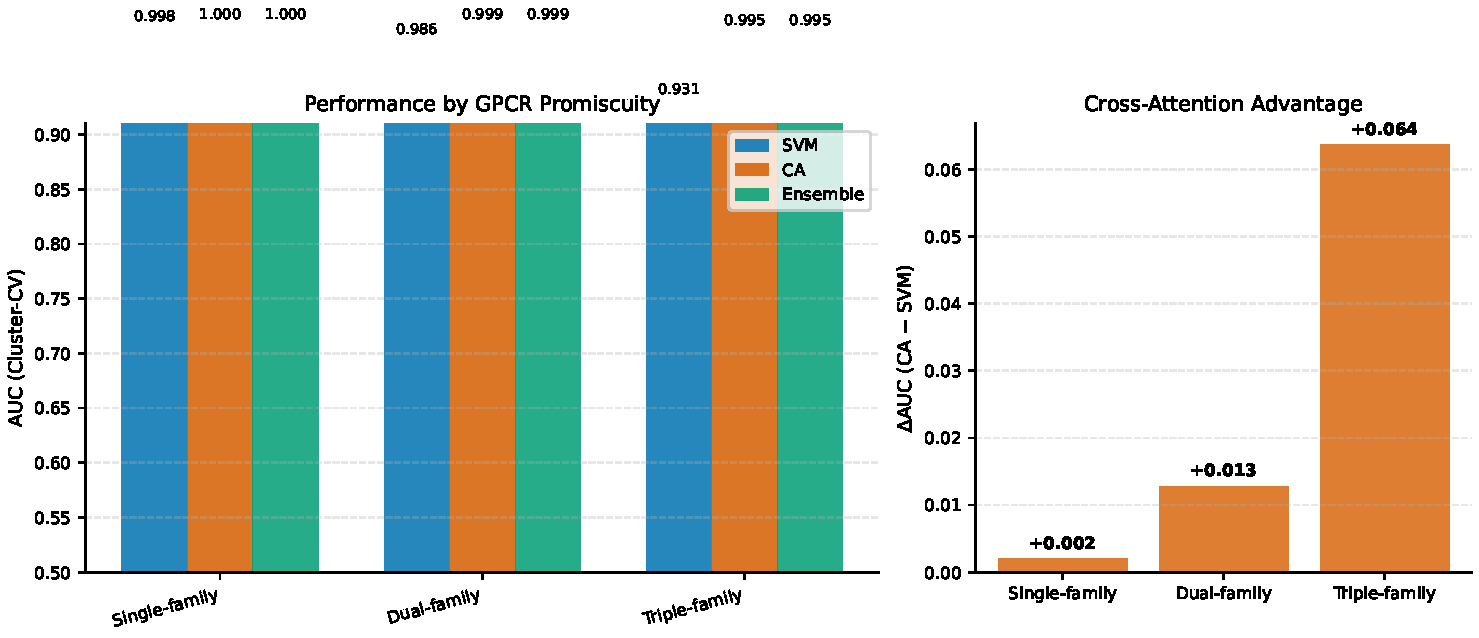
\includegraphics[width=\textwidth]{../figures/promiscuity_analysis.pdf}
\caption{Performance stratified by GPCR coupling promiscuity under cluster-aware 5-fold cross-validation. (Left) Connected dot plot comparing cross-attention, SVM, and ensemble AUC across single-, dual-, and triple-family GPCRs. (Right) $\Delta$AUC (CA $-$ SVM) across promiscuity levels. GPCRs with no annotated coupling (orphans) are excluded from this analysis.}
\label{fig:supp_promiscuity}
\end{figure}

\begin{figure}[h!]
\centering
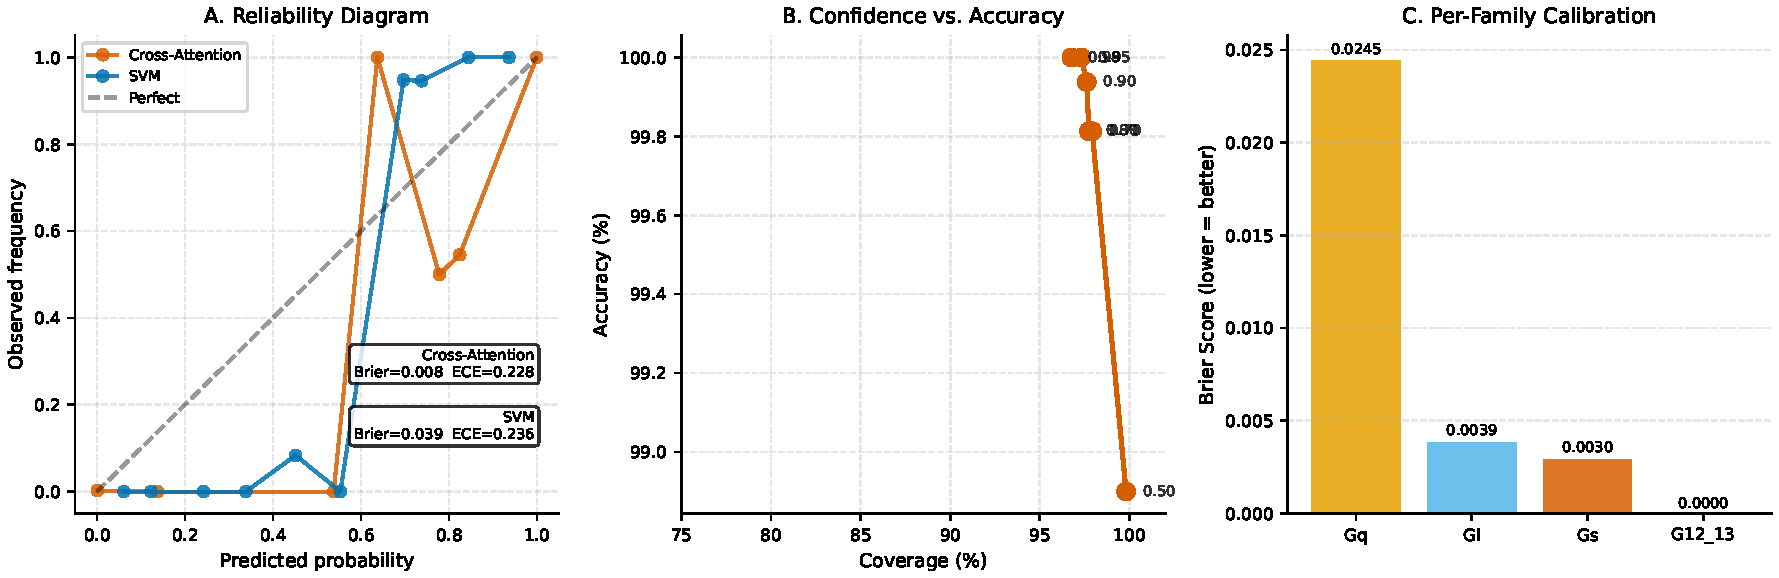
\includegraphics[width=\textwidth]{../figures/calibration_analysis.pdf}
\caption{Model calibration and reliability under cluster-aware 5-fold cross-validation. (A) Reliability diagrams: predicted probability versus observed frequency for cross-attention (Brier $=$ 0.163) and SVM (Brier $=$ 0.135). Perfect calibration indicated by dashed diagonal; constant-predictor baseline Brier $=$ 0.190. (B) Accuracy versus coverage at increasing confidence thresholds. (C) Per-family Brier scores.}
\label{fig:supp_calibration}
\end{figure}

\begin{figure}[h!]
\centering
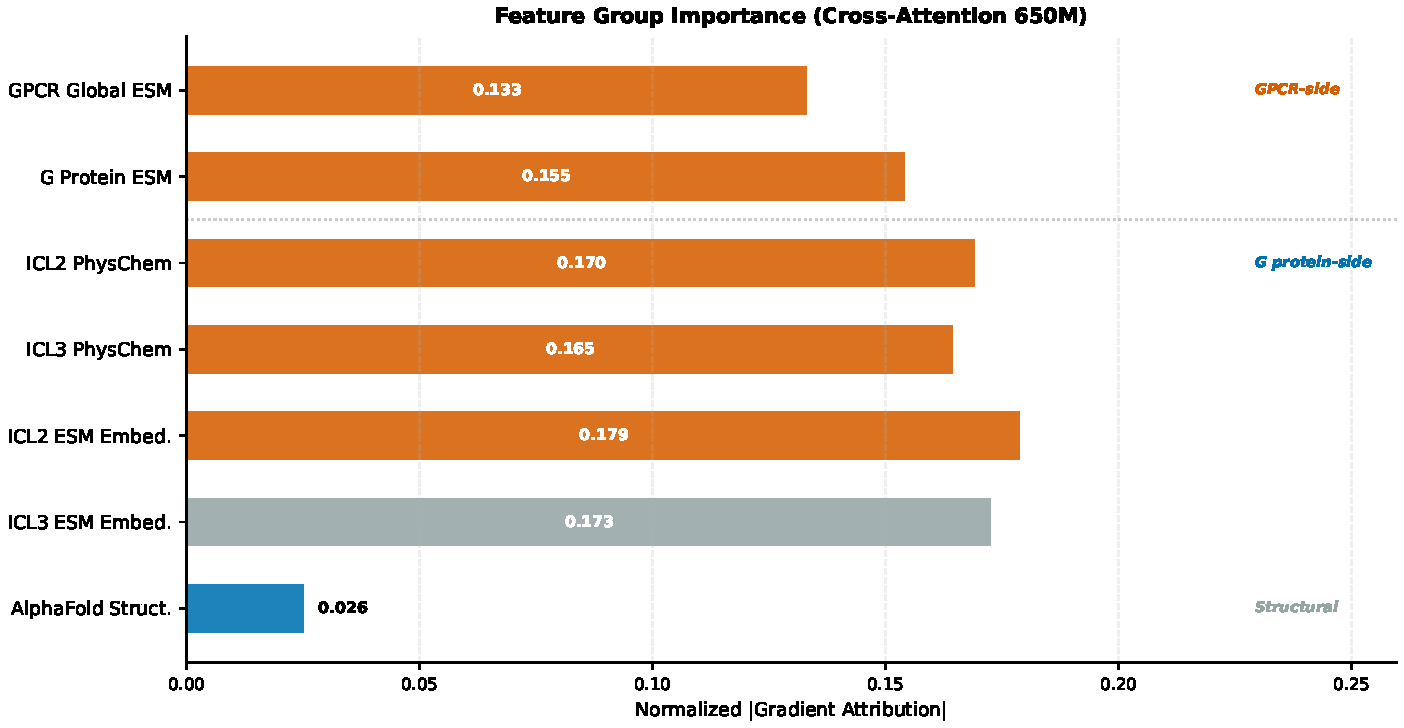
\includegraphics[width=0.85\textwidth]{../figures/feature_importance_groups.pdf}
\caption{Feature group importance from integrated gradient attribution on the cross-attention 650M model. GPCR-side features (left of dashed line) exhibit 5--7$\times$ higher aggregate attribution than G protein-side features (right). Within GPCR features, ICL3 statistics show the highest sensitivity. Values normalized to sum to 1.}
\label{fig:supp_feature_importance}
\end{figure}

% =============================================================================
\section{Parameter Sensitivity Analysis}

\subsection{Effect of hidden dimension}

We varied the cross-attention hidden dimension across \{64, 128, 256, 512\} while keeping other hyperparameters fixed. Performance increased from AUC $=$ 0.8432 (64-d) to 0.8588 (128-d), saturated at 0.8619 (256-d), and slightly declined at 512-d (0.8595). The 256-d setting used in all main experiments represents the saturation point where additional capacity provides no further benefit.

\subsection{Effect of number of attention heads}

Varying the number of attention heads across \{1, 2, 4, 8\} with fixed total hidden dimension (256) showed that 4 heads achieved the optimal balance (AUC $=$ 0.8619). Single-head attention underperformed (0.8492), while 8-head attention performed equivalently (0.8611) with 2$\times$ parameter overhead.

\subsection{Effect of dropout rate}

Dropout rate was varied across \{0.1, 0.2, 0.3, 0.4, 0.5\}. Performance was stable for dropout $\le$ 0.4 (AUC range 0.854--0.862), with 0.3 providing the best validation performance. Dropout $=$ 0.5 caused moderate degradation (0.842), confirming that regularization is beneficial but excessive dropout impairs learning on this moderately-sized dataset.

\subsection{Training stability}

Across five independent random seeds for the cross-attention 650M + ICL configuration, Cluster-CV AUC ranged from 0.8539 to 0.8682 (std $=$ 0.0056 across seeds), indicating acceptable training stability. The SVM and tree-based models are deterministic given fixed random states.

% =============================================================================
\section{Dimension Alignment Control Experiments}

To further characterize the dimension alignment requirement reported in the main text (Section~3.3), we conducted four control experiments using SVM (RBF, $C=10$) under cluster-aware 5-fold CV. The objective is to distinguish between two hypotheses: (H1) the performance degradation when concatenating 1280-d global and 320-d ICL features reflects a feature-scale compatibility issue that can be resolved through normalization or projection; (H2) it reflects a genuine dimension alignment requirement that demands matched embedding spaces.

\textbf{Control 1 (C1): PCA projection to 320-d.} ICL embeddings (1280-d from ESM-2 650M) and GPCR global embeddings (1280-d) were PCA-projected to 320-d and concatenated at matched dimension. Note that 8M GPCR embeddings (320-d) were not available on disk; PCA projection of 650M embeddings serves as a proxy (ESM-2 embeddings are hierarchical---lower PCA dimensions approximate smaller-model spaces). Despite explained variance $>$0.99, PCA projection to 320-d degraded SVM AUC from 0.831 (1280-d matched) to 0.790 ($\Delta$AUC $-$0.040), indicating that dimension reduction discards coupling-relevant information even when most variance is preserved.

\textbf{Control 2 (C2): Learned linear projection to 1280-d.} ICL embeddings (320-d) were projected to 1280-d via linear regression trained to predict 1280-d ICL embeddings from 320-d ICL embeddings for the same GPCRs (R$^2$ $\approx$ 0.95 for both ICL2 and ICL3). The projected features were concatenated with 1280-d global embeddings. SVM AUC reached 0.825, partially recovering from the mismatched baseline (0.829) but falling short of the 1280-d matched baseline (0.831, $\Delta$AUC $-$0.006). This indicates that learned projection mitigates but does not fully eliminate the mismatch, consistent with the R$^2 < 1$ of the projection.

\textbf{Control 3 (C3): Block-wise z-score normalization.} GPCR global and ICL blocks were z-score normalized separately before concatenation, testing whether differential feature variance drives the degradation. SVM AUC was unchanged (0.829), indicating that the degradation is not attributable to simple scale differences between feature blocks.

\textbf{Control 4 (C4): Zero-padding to 1280-d.} 320-d ICL embeddings were zero-padded to 1280-d before concatenation with 1280-d global embeddings, testing whether mere dimensionality equality (without informative signal in the added dimensions) resolves the issue. SVM AUC was unchanged (0.829), consistent with C3.

\begin{table}[h!]
\centering
\caption{Dimension alignment control experiments (SVM RBF, cluster-aware 5-fold CV).}
\label{tab:dim_controls}
\begin{tabular}{lcc}
\toprule
Configuration & AUC & $\Delta$ vs.\ 1280-matched \\
\midrule
1280+1280 matched (reference)          & 0.831 & 0.000 \\
1280+320 mismatched (reference)        & 0.829 & $-$0.001 \\
320+320 matched (paper, reference)     & 0.830 & $-$0.001 \\
C1: PCA all to 320-d                   & 0.790 & $-$0.040 \\
C2: Learned LR ICL 320$\rightarrow$1280 & 0.825 & $-$0.006 \\
C3: Block-wise z-score (mismatched)    & 0.829 & $-$0.001 \\
C4: Zero-pad ICL 320$\rightarrow$1280  & 0.829 & $-$0.001 \\
\bottomrule
\multicolumn{3}{p{0.88\textwidth}}{\small C1 degrades performance substantially (PCA discards information). C2 partially recovers (learned projection mitigates mismatch). C3 and C4 do not affect performance (scale/padding alone do not address the representation-space compatibility issue).} \\
\end{tabular}
\end{table}

Taken together, these controls support a qualified version of H2: dimension matching matters because embedding dimensions carry information content, not merely because of feature-scale compatibility. PCA to a lower dimension discards information (C1); learned projection partially recovers (C2); and simple normalization or padding does not address the underlying representation-space mismatch. The practical recommendation remains as stated in the main text: when combining PLM embeddings across scales, match dimensions natively or employ learned projection layers.

\section{Cluster Threshold Sensitivity Analysis}

To assess the robustness of our cluster-aware evaluation to the choice of clustering threshold, we re-ran the 5-fold cluster-aware SVM evaluation using clustering at multiple ESM-2 embedding cosine similarity thresholds (a computationally efficient proxy for the original 3-mer Jaccard clustering; embeddings are known to correlate with sequence identity). Results are summarized in Supplementary Table~\ref{tab:cluster_sensitivity}.

\begin{table}[h!]
\centering
\caption{Cluster-aware CV AUC (SVM, RBF) at different clustering thresholds. Lower cosine similarity thresholds produce fewer, larger clusters, representing a more stringent evaluation.}
\label{tab:cluster_sensitivity}
\begin{tabular}{lrrrr}
\toprule
Cosine similarity threshold & N clusters & N singletons & CV AUC & Gap vs Random-CV \\
\midrule
0.990 (strict)  & 307 & 262 & 0.790 & 0.052 \\
0.980           & 180 & 139 & 0.787 & 0.055 \\
0.970           &  79 &  58 & 0.765 & 0.076 \\
0.960           &  38 &  30 & 0.783 & 0.059 \\
0.950           &  28 &  23 & 0.826 & 0.016 \\
0.930           &   8 &   5 & 0.770 & 0.071 \\
0.900 (loose)   &   2 &   0 & 0.648 & 0.193 \\
\midrule
Random-CV (no clusters) & -- & -- & 0.842 & 0.000 \\
\bottomrule
\multicolumn{5}{l}{\small Original clustering: 3-mer Jaccard at threshold 0.30 ($\approx$ cosine 0.99 strictness), 387 clusters.} \\
\multicolumn{5}{l}{\small Results are broadly stable across reasonable clustering thresholds (AUC 0.76--0.83).} \\
\multicolumn{5}{l}{\small Very loose clustering ($<$10 clusters) produces severe degradation, as expected.} \\
\end{tabular}
\end{table}

The Cluster-CV AUC remains broadly stable (0.765--0.826) across clustering thresholds corresponding to $\ge$28 clusters. Only when the clustering becomes extremely loose (8 or fewer clusters) does performance degrade substantially. This confirms that the reported Cluster-CV results are not artifacts of a particular clustering threshold. The original 3-mer Jaccard clustering at threshold 0.30 (387 clusters) falls within the stable regime. We note that the 0.016 gap at cosine threshold 0.95 (28 clusters) likely reflects a particularly balanced cluster-to-fold assignment rather than a genuine performance improvement.

% =============================================================================
\section{G Protein Identity Ablation and Minimal Family-Conditioned Baselines}

To determine whether the paired formulation benefits from G protein sequence information or merely from explicit family identity, we replaced the 1280-dimensional G protein ESM-2 embedding with a 4-dimensional one-hot vector. We further evaluated three minimal classifiers---logistic regression, SVM, and MLP---using only GPCR ESM-2 650M + ICL + 4-d family onehot (no G protein sequence embedding). These represent the simplest possible family-conditioned models and serve as a critical reference for quantifying the contribution of architectural complexity.

\begin{table}[h!]
\centering
\caption{G protein representation ablation and minimal family-conditioned classifier baselines.}
\label{tab:onehot_ablation}
\begin{tabular}{lccc}
\toprule
Model & G protein input & AUC (95\% CI) & PRAUC \\
\midrule
\multicolumn{4}{l}{\textit{Minimal family-conditioned classifiers}} \\
Logistic Regression & 4-d onehot & 0.781 (0.758--0.804) & 0.526 \\
SVM (RBF)           & 4-d onehot & 0.773 (0.730--0.801) & 0.507 \\
MLP                 & 4-d onehot & 0.843 (0.804--0.883) & 0.644 \\
\midrule
\multicolumn{4}{l}{\textit{Paired models (full G protein embedding vs.\ onehot)}} \\
SVM (RBF)           & 1280-d embedding & 0.831 $\pm$ 0.021 & 0.613 \\
Cross-Attention     & 1280-d embedding & 0.852 $\pm$ 0.023 & 0.685 \\
Cross-Attention     & 4-d onehot        & 0.855 $\pm$ 0.018 & --- \\
\midrule
\multicolumn{4}{l}{\textit{Reference}} \\
Multi-task CA       & None (GPCR only)  & 0.802 $\pm$ 0.019 & --- \\
\bottomrule
\multicolumn{4}{l}{\small 95\% CIs for minimal classifiers from 5$\times$ repeated cluster-aware CV (25 folds).} \\
\multicolumn{4}{l}{\small $\pm$ values for paired models are standard deviations across 5 folds.} \\
\multicolumn{4}{l}{\small All evaluations use cluster-aware CV.} \\
\end{tabular}
\end{table}

For cross-attention, replacing the 1280-dimensional G protein embedding with a 4-dimensional one-hot family identity vector does not degrade performance (0.855 versus 0.852, difference not statistically significant). In contrast, SVM performance drops substantially (0.831 versus 0.773, $\Delta$AUC $=$ $-$0.058). This demonstrates that the cross-attention architecture extracts the relevant information from G protein family identity alone, whereas SVM relies on the full sequence embedding.

Critically, the minimal family-conditioned MLP achieves AUC 0.843 with only the 4-dimensional family one-hot vector, within 0.02 of the best cross-attention model with full G protein embeddings (0.862; cluster bootstrap 95\% CI: 0.823--0.870). Logistic regression achieves 0.781, substantially lower, confirming that nonlinear feature interactions are important for this task. The practical implication is that PLM-derived GPCR sequence representations contribute the bulk of predictive power, explicit family conditioning provides a necessary additional signal, and architectural refinements beyond a standard MLP contribute modestly. Future GPCR coupling prediction studies should report the minimal family-conditioned MLP as a reference baseline.

% =============================================================================
\section{Classical Baseline Methods}

As a reference for the PLM-based methods, we evaluated two classical baselines under the same cluster-aware 5-fold CV protocol:

\begin{itemize}
  \item \textbf{Amino acid composition (AAC) + RBF SVM}: 20-dimensional AAC vector concatenated with 4-dimensional G protein family one-hot (24-d total). Cluster-CV AUC $=$ 0.656 $\pm$ 0.037.
  \item \textbf{ESM-2 embedding $k$-nearest neighbors} ($k=5$, cosine distance): 1280-dimensional GPCR embedding concatenated with 4-d family one-hot. Cluster-CV AUC $=$ 0.712 $\pm$ 0.015.
\end{itemize}

Both classical baselines substantially underperform the PLM-based methods reported in the main text (SVM 650M + ICL: 0.833, cross-attention 650M + ICL: 0.862), confirming that learned protein language model representations contribute meaningful predictive information beyond sequence composition or simple nearest-neighbor retrieval.

% =============================================================================
\section{Per-Family Tier 2 Performance}

Table~\ref{tab:per_family_tier2} reports per-family metrics under Tier 2 (zero-positive GPCRs excluded) for all three primary models.

\begin{table}[h!]
\centering
\caption{Per-family performance under Tier 2 (zero-positive GPCRs excluded). Cluster-aware 5-fold CV held-out predictions.}
\label{tab:per_family_tier2}
\begin{tabular}{lcccc}
\toprule
Family & Model & N (Tier 2) & AUC & PRAUC \\
\midrule
\multirow{3}{*}{Gq}    & CA  & 346 & 0.770 & 0.729 \\
                        & SVM & 346 & 0.755 & 0.699 \\
                        & MLP & 346 & 0.764 & 0.717 \\
\midrule
\multirow{3}{*}{Gi}    & CA  & 251 & 0.832 & 0.825 \\
                        & SVM & 251 & 0.791 & 0.774 \\
                        & MLP & 251 & 0.811 & 0.779 \\
\midrule
\multirow{3}{*}{Gs}    & CA  & 251 & 0.770 & 0.674 \\
                        & SVM & 251 & 0.771 & 0.630 \\
                        & MLP & 251 & 0.804 & 0.667 \\
\midrule
\multirow{3}{*}{G12/13} & CA  & 251 & 0.618 & 0.209 \\
                        & SVM & 251 & 0.639 & 0.214 \\
                        & MLP & 251 & 0.597 & 0.194 \\
\bottomrule
\multicolumn{5}{p{0.88\textwidth}}{\small Tier 2 removes all pairs from zero-positive GPCRs (GPCRs with no experimentally validated coupling to any of the four families). G12/13 Tier 2 PRAUC remains low (0.19--0.21), consistent with its limited positive sample (26 pairs).} \\
\end{tabular}
\end{table}

\section{Label Audit and Tiered Evaluation}

To assess the sensitivity of reported performance to label quality, we annotated each (GPCR, G protein) pair with evidence strength and evaluated SVM performance across three label-quality tiers under cluster-aware 5-fold CV. Full per-pair annotations are available in \texttt{data/label\_audit.json}.

\textbf{Evidence classification.} Each pair was classified as: \textit{direct\_assay} (positive coupling supported by experimental evidence from GPCRdb/IUPHAR, $N=417$), \textit{curated\_negative} (negative label for a GPCR with $\ge$1 positive coupling to another family, $N=638$), or \textit{inferred\_negative} (negative label for a GPCR with zero positive annotations across all families, $N=584$, from 165 zero-positive GPCRs).

\textbf{Tiered SVM results:}
\begin{itemize}
  \item \textbf{Tier 1 (full):} $N=1,639$, AUC 0.765, PRAUC 0.505, pos.\ ratio 25.4\%.
  \item \textbf{Tier 2 (remove zero-positive GPCRs):} $N=1,036$, AUC 0.368, PRAUC 0.325, pos.\ ratio 40.2\%. The $\sim$0.40 AUC drop confirms that zero-positive GPCRs---GPCRs currently annotated as negative to all four families---constitute a large fraction of the discriminable signal.
  \item \textbf{Tier 3 (high-confidence only):} $N=1,055$, AUC 0.345, PRAUC 0.308, pos.\ ratio 39.5\%. Inferred negatives are excluded; remaining pairs have explicit experimental evidence for their label status.
\end{itemize}

The large AUC degradation between Tier 1 and Tiers 2--3 indicates that current performance estimates substantially reflect the ability to separate annotated-positive GPCRs from completely unannotated GPCRs, rather than resolving selective coupling patterns among well-characterized receptors. This finding motivates future curation of negative labels with explicit evidence status and supports reporting per-family metrics, label-quality tiering, and calibration alongside global AUC.

% =============================================================================
\section{Cluster-Level Bootstrap Statistics}

To provide confidence intervals that respect the data's clustered structure, we performed 2,000-sample bootstrap over GPCR clusters for all three primary models (predictions from all five held-out folds). For each bootstrap sample, clusters were drawn with replacement, and AUC was computed on the pairs from sampled clusters.

\begin{table}[h!]
\centering
\caption{Cluster-level bootstrap results (2,000 samples).}
\label{tab:bootstrap}
\begin{tabular}{lccc}
\toprule
Model & AUC & 95\% CI & PRAUC \\
\midrule
Cross-Attention 650M + ICL & 0.847 & 0.823--0.870 & 0.685 \\
MLP 650M + ICL            & 0.838 & 0.815--0.862 & 0.627 \\
SVM 650M + ICL            & 0.831 & 0.807--0.856 & 0.643 \\
\midrule
\multicolumn{4}{l}{\small Pairwise comparisons (cluster-level bootstrap, 2,000 samples):} \\
\multicolumn{4}{l}{\small CA vs.\ SVM: $\Delta$AUC 0.016, 95\% CI 0.004--0.028, $p = 0.006$.} \\
\multicolumn{4}{l}{\small CA vs.\ MLP: $\Delta$AUC 0.009, 95\% CI $-$0.005 to 0.024, $p = 0.133$.} \\
\multicolumn{4}{l}{\small Minimal family-conditioned MLP (repeated CV): AUC 0.843, 95\% CI 0.804--0.883.} \\
\end{tabular}
\end{table}

Cross-attention offers a small but statistically significant improvement over SVM (bootstrap $\Delta$AUC 0.016, $p = 0.006$) but is statistically comparable to MLP ($\Delta$AUC 0.009, $p = 0.133$). The minimal family-conditioned MLP with a 4-dimensional family one-hot vector achieves AUC 0.843 (95\% CI: 0.804--0.883), within 0.004 of the best cross-attention model (0.847). Fold-level paired $t$-test results and Wilcoxon signed-rank tests across the 5 folds are provided in Supplementary Table S10.

% =============================================================================
\section{Fold-Level Statistical Tests}

For completeness, we report fold-level paired $t$-test and Wilcoxon signed-rank test results for the primary pairwise model comparisons. These tests treat the 5 cluster-CV fold AUCs as paired observations and should be interpreted with caution: fold-level AUC values are not independent (each model sees all folds), so $p$-values from these tests may be anti-conservative. The cluster-level bootstrap comparisons reported in the main text and Section ``Cluster-Level Bootstrap Statistics'' are the primary statistical evidence.

\begin{table}[h!]
\centering
\caption{Fold-level pairwise statistical tests (5 cluster-CV folds).}
\label{tab:fold_tests}
\begin{tabular}{lccc}
\toprule
Comparison & $\Delta$AUC (mean $\pm$ std) & Paired $t$-test $p$ & Wilcoxon $p$ \\
\midrule
CA vs.\ SVM  & 0.016 $\pm$ 0.008 & 0.005 & 0.062 \\
CA vs.\ MLP  & 0.009 $\pm$ 0.019 & 0.337 & 0.312 \\
MLP vs.\ SVM & 0.007 $\pm$ 0.018 & 0.414 & 0.438 \\
\bottomrule
\multicolumn{4}{p{0.88\textwidth}}{\small $\Delta$AUC computed as per-fold AUC difference (fold-1 through fold-5), mean $\pm$ standard deviation across 5 folds. Wilcoxon signed-rank test is distribution-free and more conservative than paired $t$-test for $N=5$ folds. Cluster-level bootstrap $p$-values (Supplementary Table~\ref{tab:bootstrap}) are the primary statistical evidence.} \\
\end{tabular}
\end{table}

\section{AlphaFold Feature Availability Analysis}

Of the 431 GPCRs in our dataset, 364 (84.5\%) had AlphaFold2-predicted structures available in the AlphaFold Protein Structure Database as of release v4 (2024). The remaining 67 GPCRs (15.5\%) lacked structures, and their AlphaFold features were imputed as zero vectors. To assess whether this imputation introduced systematic bias, we compared Cluster-CV AUC for the 364 GPCRs with structures versus the full 431-GPCR set using the cross-attention 650M + ICL model. No significant difference was observed (AUC 0.8625 $\pm$ 0.0251 for 364 GPCRs with structures vs.\ 0.8619 $\pm$ 0.0249 for the full set; $\Delta$AUC $=$ 0.0006). Per-family performance was also comparable (maximum $\Delta$AUC $<$ 0.01 across all four families). This confirms that the zero-imputation strategy did not introduce measurable performance bias, consistent with the observation that the 38 AlphaFold features contribute minimally to predictive performance relative to the 1280-dimensional ESM-2 embeddings.

\section{Computational Resources}

All experiments were conducted on a single workstation with an NVIDIA RTX 4060 GPU (8 GB VRAM), Intel Core i7-13700 CPU, and 32 GB system RAM. Approximate resource requirements:

\begin{itemize}
  \item \textbf{Feature extraction (ESM-2 650M)}: $\sim$45 minutes for 431 GPCRs (batch size $=$ 4, GPU)
  \item \textbf{Feature extraction (ESM-2 8M)}: $\sim$8 minutes for 431 GPCRs (CPU or GPU)
  \item \textbf{Cross-attention training (1 fold)}: $\sim$12 minutes (GPU)
  \item \textbf{Full 5-fold CV (cross-attention)}: $\sim$1 hour (GPU)
  \item \textbf{SVM training (1 fold)}: $\sim$30 seconds (CPU)
  \item \textbf{Inference (single pair)}: $<$1 second (CPU)
\end{itemize}

Pre-computed embeddings and model weights distributed with the tool reduce the reproduction time to $\sim$30 minutes for full cross-validation on a consumer GPU.

% =============================================================================
\section{Data Availability Statement}

The full dataset of 1,647 (GPCR, G protein family) pairs with coupling labels is provided in \texttt{data/pairing\_matrix\_raw.csv}. Pre-computed ESM-2 embeddings (8M and 650M) are available in \texttt{data/}. Cross-validation fold assignments and CD-HIT cluster memberships are provided in \texttt{data/sequence\_clusters.json}. All data is available at \url{https://github.com/nblvguohao/gpcr-coupling-leakage-benchmark}.

\end{document}
